\documentclass[11pt,oneside,a4paper]{article}
\usepackage{graphicx}
\usepackage{booktabs}
\usepackage{caption}
\usepackage{subcaption}
\usepackage{amsmath}
\usepackage{amsfonts}
\usepackage{amssymb}
\usepackage{lscape}
\usepackage{psfrag}
\usepackage[usenames]{color}
\usepackage{bbm}
\usepackage[update]{epstopdf}
\usepackage[bookmarks,pdfstartview=FitH,a4paper,pdfborder={0 0 0}]{hyperref}
\usepackage{verbatim}
\usepackage{listings}
\usepackage{textcomp}
\usepackage{course}
\usepackage{fancyhdr}
\usepackage{multirow}
\usepackage{algorithm}
\usepackage{algcompatible}
\usepackage[noend]{algpseudocode}
\pagestyle{fancy}
\usepackage{tikz}
\usepackage{xcolor}
\usepackage[title]{appendix}

\renewcommand{\sectionmark}[1]{\markboth{#1}{#1}}
\renewcommand{\subsectionmark}[1]{\markright{#1}}

\fancyhf{}
\fancyhead[RO]{\nouppercase{\footnotesize\sc\rightmark\ \hrulefill\ \thepage}}
\fancyhead[RE]{\nouppercase{\footnotesize\sc\thepage\ \hrulefill\ }}
\renewcommand{\headrulewidth}{0pt}

\makeatletter
\def\cleardoublepage{\clearpage\if@twoside \ifodd\c@page\else%
\hbox{}%
\thispagestyle{empty}%
\clearpage%
\if@twocolumn\hbox{}\clearpage\fi\fi\fi}
\makeatother


\renewcommand{\topfraction}{0.9}  % max fraction of floats at top
\renewcommand{\bottomfraction}{0.8} % max fraction of floats at bottom
% Parameters for TEXT pages (not float pages):
\setcounter{topnumber}{2}
\setcounter{bottomnumber}{2}
\setcounter{totalnumber}{4}            % 2 may work better
\setcounter{dbltopnumber}{2}           % for 2-column pages
\renewcommand{\dbltopfraction}{0.9}    % fit big float above 2-col. text
\renewcommand{\textfraction}{0.07}     % allow minimal text w. figs
% Parameters for FLOAT pages (not text pages):
\renewcommand{\floatpagefraction}{0.7}  % require fuller float pages
% N.B.: floatpagefraction MUST be less than topfraction !!
\renewcommand{\dblfloatpagefraction}{0.7} % require fuller float pages

\sloppy

\widowpenalty=10000
\clubpenalty=10000

\edef\today{%\number\day\
\ifcase\month\or
January\or February\or March\or April\or May\or June\or July\or
August\or September\or October\or November\or December\fi\ \number\year}
\title{\vspace*{40.0mm}
  \bf\sf Parallel Hashing
         \vspace*{20.0mm} \\
  \vspace*{40.0mm}
  %\vspace{-20mm}\framebox{DRAFT VERSION}\vspace{20mm} \\
  \Large\bf\sf Program for Undergraduate Research \vspace*{20.0mm}}
\author{\sf Kamer Kaya, Fatih Tasyaran,Kerem Yildirir,Hakan Ogan Alpar,Ali Osman Berk}
\date{\sf \today}

\begin{document}

\begin{figure}
  \parbox[t]{40mm}{
    \begin{flushleft}
      
\includegraphics[height=25mm]{pure.png}
    \end{flushleft}}
    \hspace{7cm}
  \parbox[t]{40mm}{
    \begin{flushright}
      
\includegraphics[height=25mm]{sabanj.png}
    \end{flushright}}
\end{figure}

\maketitle
\thispagestyle{empty}
\raggedbottom

\cleardoublepage
\pagenumbering{roman}
\setcounter{tocdepth}{2}
\tableofcontents


\section{Introduction}
\par Searching is one of the most important problems of computer science and it is used extensively in many areas such as cryptography and network security. Hash functions are one-way functions that map an input value to another value. Randomness is essential in hashing because it is not desired to have multiple values resulting in the same hash value. Hashing is also used in  data structures where we use the hashed values as indexes of a table  and keep the value in the index of a table determined by hash function. This property allows us to do search, insert, delete operations in O(1) time. In this work, we introduce using SIMD instructions by Intel in hash functions to generate hash values in parallel by using different data points in a single instruction. Section 2 introduces the  SIMD instructions,  section 3 discusses the two different hashing approaches we worked on , section 4 presents the improvement we achieved and section 5 presents applications for our work.
\section{Intel SIMD Instructions}
SIMD is an instruction set available mostly on all current processors. In this project we used AVX (Advanced Vector Extension) and AVX2 instructions which are available for Intel processors since Sandy Bridge architecture. With AVX instructions, it is possible to process 128 bits of data in registers on parallel, with AVX2 this increased to 256 bits, meaning that we can do simple arithmetic and logical operations of 8 32-bit integers at the same time. The SIMD instructions we used on this project and their descriptions could be found in Appendix A.
\section{Hashing Strategies}
As our hash functions, we used Multiply-Shift Hash, MurMurHash3  and Tabular Hash. Pseudocodes of these functions can be found in Appendix B. For each hash function, we have developed our work under 2 models; Model 1, one data multiple hash, where we generate multiple hash values from a single data sample, and Model 2, one data one hash, where we generate only one hash value using the same random seed for a single data sample. For both models we implemented the hash functions with SIMD instructions in simple arithmetic and logical operations. This way we were able to process 8 32-bit integers in parallel.
\subsection{Model 1}
\begin{figure}[H]
\centering
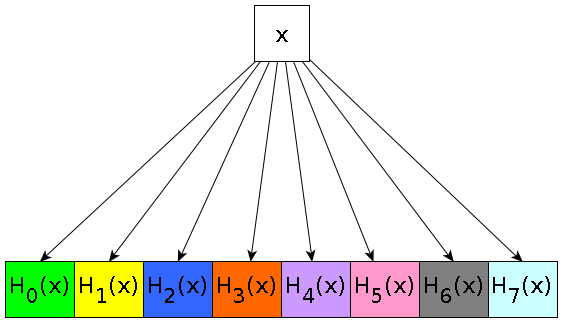
\includegraphics[width=0.5\textwidth]{one_data_multi_hash.png} 
\caption{Illustration of Model 1}
\end{figure}
First model computes 8 hash values for a single given input. We apply the hash function using 8 different random seeds and do all the operations using these random 8 values. We fill an array of size 8 with our input value and apply the operation with 8 different random seeds. This model is especially useful for algorithms like Count-Min Sketch where we keep multiple hash values for a single element. 
\subsection{Model 2}
\begin{figure}[H]
\centering		
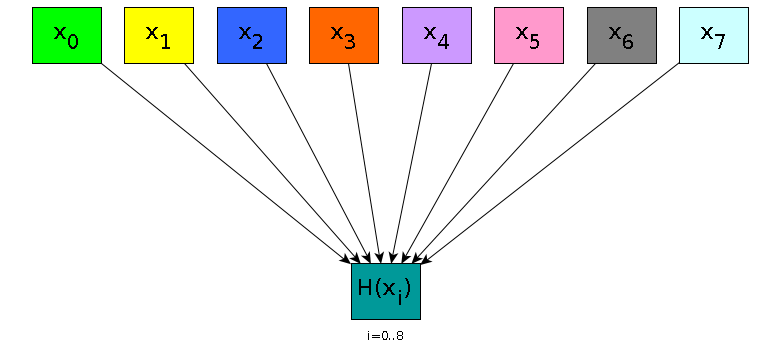
\includegraphics[width=0.7\textwidth]{multi_data_single_hash.png} 
\caption{Illustration of Model 2}
\end{figure}
Second model computes 8 hash values for given 8 inputs, using the same random seed for all data points. This approach could be seen as overriding the data length a register can hold, which is 256 bits, by carrying 8 different 32-bit value to get 8 different 32-bit hash result by single instruction, in parallel. Using this approach, the goal is to achieve 8 hash values in a time of 1 hash value without SIMD instructions. This approach could be useful in applications like bloom filter, where every element needs one hash to check membership to a set.
\section{Experiment and Results}
\section{Future Work}
In the future, we plan to use our hash functions with SIMD instructions in probabilistic data structures and algorithms such as HyperLogLog, Bloom Filter and Count-Min Sketch. These algorithms are very useful in estimating frequencies in large data streams.  We believe that parallelizing the hashing operations in these algorithms  will provide great amount of speedup in frequency estimation. 
\subsection{HyperLogLog}
HyperLogLog hashes every key to a bit stream and then approximates the distinct element number of the hashed set by bit stream's prefixes. To do this, HyperLogLog uses the same hash function for all keys to be hashed. With this property, HyperLogLog is suitable for multiple data, one hash approach. 
Implementing SIMD instructions on a HyperLogLog could achieve great speedup as the HyperLogLog works in a one pass over data manner, only counting hash values..  
\subsection{Bloom Filter}
As mentioned earlier, bloom filter is one of the well suited applications for multiple data - one hash approach. To open up, bloom filter is a membership query which hashes keys to hash values and map them in a bit vector. With a bloom filter employing a SIMD instruction including hash function, it would be possible to answer 8 membership queries at once.
\subsection{Count-Min Sketch}
Count-min sketch is a perfectly well suited application to use with one data multiple hash approach. Since a count-min sketch is basically a 2 dimensional matrix, the rows of which are 1 dimensional hashtables. To insert an element to a sketch (i.e. counting it) requires different hash values for each row of the count-min sketch. By using  SIMD instructions, calculatıng hash values for all rows a sketch at a time could achieve a promising speed-up for the hashing phase of a count-min sketch.
\cleardoublepage
\pagenumbering{arabic}

\cleardoublepage


\bibliographystyle{ieeetr}
\bibliography{mybib.bib}
\begin{appendices}
\section{SIMD Instructions Used in Project}
\subsection{Load-Extract Instructions}
\textcolor{blue}{\_\_m256i} \_mm256\_load\_si256 (\textcolor{blue}{\_\_m256i const *} \textcolor{green}{mem\_addr})
\par Load 256-bits of integer data from memory into dst. mem\_addr must be aligned on a 32-byte boundary.
\par
\textcolor{blue}{\_\_m256i} \_mm256\_loadu\_si256 (\textcolor{blue}{\_\_m256i const *} \textcolor{green}{mem\_addr})
\par Load 256-bits of integer data from memory into dst.mem\_addr does not need to be aligned on any particular boundary.
\par
\textcolor{blue}{ \_\_int32} \_mm256\_extract\_epi32 ( \textcolor{blue}{ \_\_m256i} \textcolor{green}{a}, \textcolor{blue}{const int} \textcolor{green}{b})
\par Add 4 packed to 256-bit side by side 64-bit integers in a and b, and store the results in dst.
\par
\textcolor{blue}{ \_\_m256i} \_mm256\_set1\_epi32 ( \textcolor{blue}{ int} \textcolor{green}{a})
\par Broadcast 32-bit integer a to all elements of dst.
\par 
\subsection{Bitwise Instructions}
\textcolor{blue}{ \_\_m256i} \_mm256\_slli\_epi64 ( \textcolor{blue}{ \_\_m256i} \textcolor{green}{a}, \textcolor{blue}{int} \textcolor{green}{imm8})
\par Shift packed 64-bit integers in a left by imm8 while shifting in zeros, and store the result in dst.
\par
\textcolor{blue}{ \_\_m256i} \_mm256\_slri\_epi64 ( \textcolor{blue}{ \_\_m256i} \textcolor{green}{a}, \textcolor{blue}{int} \textcolor{green}{imm8})
\par Shift packed 64-bit integers in a right by imm8 while shifting in zeros, and store the result in dst.
\par
\textcolor{blue}{ \_\_m256i} \_mm256\_shuffle\_epi32 ( \textcolor{blue}{ \_\_m256i} \textcolor{green}{a}, \textcolor{blue}{int} \textcolor{green}{imm8})
\par Shuffle 32-bit integers in a within 128-bit lanes using the control in imm8, and store the results in dst.
\subsection{Arithmetic Instructions}
\textcolor{blue}{ \_\_m256i} \_mm256\_add\_epi32 ( \textcolor{blue}{ \_\_m256i} \textcolor{green}{a}, \textcolor{blue}{ \_\_m256i} \textcolor{green}{b})
\par Add 8 packed to 256-bit side by side 32-bit integers in a and b, and store the results in dst.
\par
\textcolor{blue}{ \_\_m256i} \_mm256\_add\_epi64 ( \textcolor{blue}{ \_\_m256i} \textcolor{green}{a}, \textcolor{blue}{ \_\_m256i} \textcolor{green}{b})
\par Add 4 packed to 256-bit side by side 64-bit integers in a and b, and store the results in dst.
\par
\textcolor{blue}{ \_\_m256i} \_mm256\_sub\_epi64 ( \textcolor{blue}{ \_\_m256i} \textcolor{green}{a}, \textcolor{blue}{ \_\_m256i} \textcolor{green}{b})
\par Subtract packed 64-bit integers in b from 64-bit integers in a, and store the result in dst.
\par
\textcolor{blue}{ \_\_m256i} \_mm256\_mullo\_epi32 ( \textcolor{blue}{ \_\_m256i} \textcolor{green}{a}, \textcolor{blue}{ \_\_m256i} \textcolor{green}{b})
\par Multiply the packed 32-bit integers in a and b, producing intermediate 64-bit integers, and store the low 32 bits of the intermediate integers in dst.
\par
\subsection{Logical Instructions}
\textcolor{blue}{ \_\_m256i} \_mm256\_and\_si32 ( \textcolor{blue}{ \_\_m256i} \textcolor{green}{a}, \textcolor{blue}{ \_\_m256i} \textcolor{green}{b})
\par Compute the bitwise AND of 256 bits integer represented data in a and b and store the result in dst.
\par
\textcolor{blue}{ \_\_m256i} \_mm256\_xor\_si256 ( \textcolor{blue}{ \_\_m256i} \textcolor{green}{a}, \textcolor{blue}{ \_\_m256i} \textcolor{green}{b})
\par Compute the bitwise XOR of 256 bits integer represented data in a and b and store the result in dst.
\par


\section{Hash Functions Used in Project}
\subsection{Multiply-Shift Hash}
\begin{algorithm}[H]
\begin{algorithmic}[1]
\Function {Multiply-Hash}{x}

\State{2 randomly sampled 64 bit integers $m_a$,$m_b$ ; }


\Return {$(m_a*(uint\_64)*x + m_b ) >> 32$}
\EndFunction
\end{algorithmic}


\end{algorithm}



\subsection{MurMurHash3}
\begin{algorithm}[H]
\begin{algorithmic}[1]
\Function{Murmur3}{key, len, seed}
   % //Note: In this version, all integer arithmetic is performed 
    %//with unsigned 32 bit integers. In the case of overflow, 
   % //the result is constrained by the application 
%    //of modulo 232 arithmetic.

    \State c1 = 0xcc9e2d51
    \State c2 = 0x1b873593
    \State r1 = 15
    \State r2 = 13
   \State  m = 5
    \State n = 0xe6546b64

    \State hash  =  seed

    \For {each fourByteChunk of key}
         \State  k ← fourByteChunk

          \State k = k * c1
          \State k = (k ROL r1)
          \State k = k * c2

          \State hash = hash XOR k
          \State hash = (hash ROL r2)
          \State hash = hash * m + n
	\EndFor        
	
	 \Comment{ Endian swapping is only necessary on big-endian machines.}

   \For {each remaining byte in key}

  \State      remainingBytes = SwapEndianOrderOf(remainingBytesInKey)

         \State  remainingBytes = remainingBytes * c1
          \State remainingBytes = (remainingBytes ROL r1)
          \State remainingBytes = remainingBytes * c2

         \State  hash = hash XOR remainingBytes
\EndFor
      \State hash = hash XOR len

     \State  hash = hash XOR (hash SHR 16)
      \State hash = hash * 0x85ebca6b
      \State hash = hash XOR (hash SRH 13)
      \State hash = hash * 0xc2b2ae35
      \State hash = hash XOR (hash SHR 16)
    \EndFunction
\end{algorithmic}
\end{algorithm}

\subsection{Tabular Hash}
\end{appendices}

\end{document}
